\section{Observing}
Whelp, if you're reading this, I can only assume it's because you're about to irreparably mess up your week by staying up until heinous hours of the morning. Enjoy. 

\subsection{Observing logs}
If you're observing, you should keep a log that tracks what you did, when you did it, weather conditions, seeing, etc. If something goes wrong, write it down. This may be important down the line! Nothing is too unimportant to jot down. If you're in doubt, just write it down. 

\subsection{There's extra time! Or I ran out of time!}
\subsubsection{Extra time}
If your observing program provided extra targets, take a look at their RAs before you begin the night. Look at the schedule to see when you're observing objects with similar RA. If you're ahead of schedule while you're doing these, go ahead and add in the extra! If you don't know what objects to add, you can always repeat observations. No one will ever be mad about this. The most important thing is to check that the RA for the additional observation makes sense for the current time, and the easiest way to do this is to make sure it's close to the RA of the object(s) you most recently observed. 

\subsubsection{Ran out of time}
Nothing you can really do about this. If you've hit morning and you haven't observed everything, that's that. If it's the middle of the night and you're behind schedule, you can make some decisions to skip targets. If you know the weather is going to be bad, it doesn't hurt to find out which objects are lowest priority. Always make a note in the observing log if you chose to skip something, and write down why. It's probably not your fault---the schedule may have been a bit off, or weather forced you to close the dome. No one will criticize you for this! These things are out of your control. 

\subsection{Remote}
\subsubsection{Before you begin the night...}
There are a few things you need to do before you begin the night. First, make sure you have all the necessary software installed and you know how to access all in-browser GUIs. You might need:
\begin{itemize}
    \item A VPN client. I use Cisco AnyConnect (at the time of writing this, Texas A\&M provided this software, so any instructional VPN-related screenshots will be using Cisco AnyConnect on an Ubuntu system). If you're an A\&M affiliate, you can get it through \href{connect.tamu.edu}{connect.tamu.edu}. You \textit{must} have Duo set up to do this. I spent like, two weeks trying to figure out why I couldn't get the software until I realized it was because I wasn't getting push notifications from Duo on my phone. 
    \item A VNC viewer. \href{https://www.realvnc.com/en/connect/download/viewer/}{Real VNC} is nice and it is free. 
    \item A stable internet connection. If you're doubtful of your home internet, cut your losses and go to your office. Logging back in to everything every time you lose connection will be extremely annoying. 
    \item Something(s) to keep yourself awake. Food, caffeine, music, games, etc. Observing is your priority though, so whatever it is, make sure you can drop it if you need to. For example, I do not recommend League of Legends, but I do recommend \href{https://www.stardewvalley.net/}{Stardew Valley}. A lot of people get work done during the night, but personally, I am incapable of being useful past 10:00 PM. 
\end{itemize}
\par
Second, it helps to organize your scripts/plan in advance. Do whatever you want, but I like to put scripts in separate folders for $\sim1$ hr blocks of time so I don't have to think about where/when all my targets are at night when my brain is running on steam. 

\subsubsection{CTIO/DECam}
\par
You should always know what the local time is. For CTIO, the time is the same as the \href{https://time.is/Santiago}{time in Santiago, Chile}. \\

In general, in this section, usernames/passwords/addresses will be obscured or not provided. You should get these from support. First, make sure you have installed:
\begin{itemize}
    \item A VPN client
    \item A VNC viewer
\end{itemize}

You can join the Zoom call any time between now and when you need to request observer permissions. If you have trouble with something, join the Zoom call and ask for help! \\

The first thing you need to open in your computer is your VPN. You need to do this to access the network at CTIO. Log in like in Figure \ref{fig:vpn}, but get your address, group, username, and password from support. \\

\begin{figure}[h!]
    \centering
    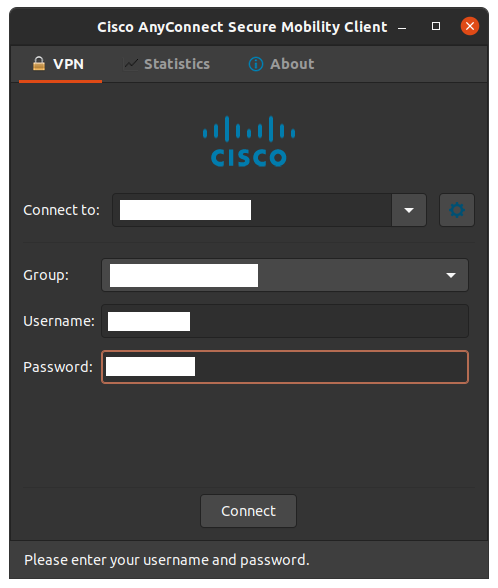
\includegraphics[width=0.6\textwidth]{figs/observing/vpn.png}
    \caption{This is what your VPN window should look like for DECam, if you're using Cisco AnyConnect.}
    \label{fig:vpn}
\end{figure}

Open up your VNC viewer. Enter the address and password. RealVNC will save this information for next time. The VNC viewer allows you to remotely use a computer at CTIO. \\

I think it's also nice to open the \href{http://www.ctio.noao.edu/noao/content/ctio-external-webcam}{CTIO external webcams}. It's the only view of the sky at CTIO you'll get all night. Plus, it's a quick way to check the weather. A slightly less quick, but more quantitative way to check the weather is to use the \href{https://noirlab.edu/science/observing-noirlab/weather-webcams/cerro-tololo/environmental-conditions}{CTIO Site Environmental Conditions page}.\\
\par
Now, open the \href{http://system1.ctio.noao.edu:7001/apps/}{SISPI GUIs}. You'll see a bunch of options, like in Figure \ref{fig:sispi}. If you're not on the VPN, you won't be able to access this page. Open one of apps in a new tab and enter the username and password provided by support. If it's not working and you've copied and pasted the login info in to the text boxes, try typing it in by hand. This has been an issue for me in the past, I'm unsure if it's inherent to the software, or if it's a browser issue, or something else. \\ 

\begin{figure}
    \centering
    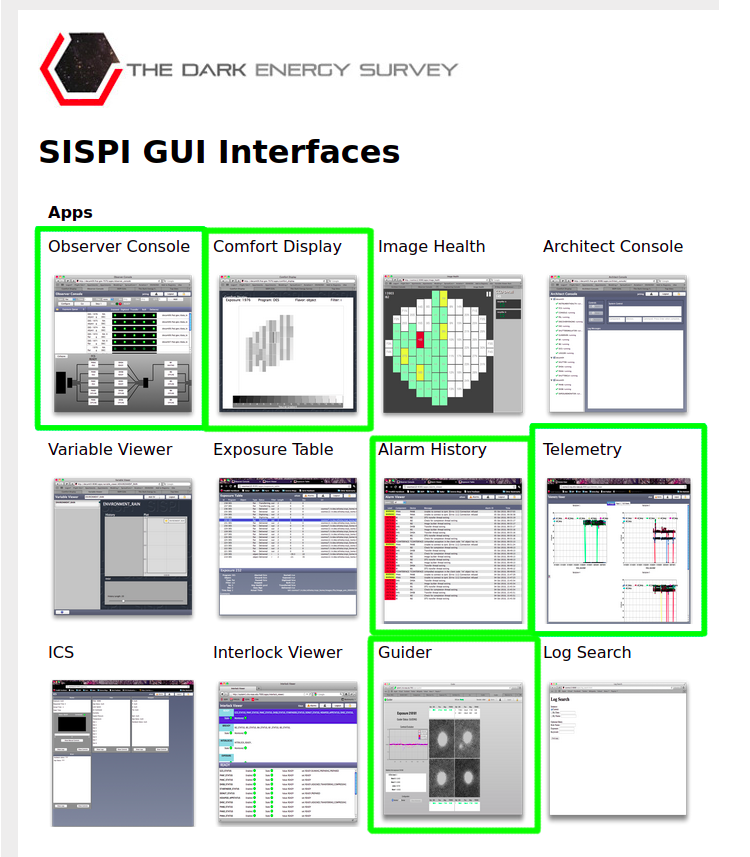
\includegraphics[width=0.5\textwidth]{figs/observing/sispi.png}
    \caption{The SISPI GUIs, with the important ones (or so I think) highlighted in green.}
    \label{fig:sispi}
\end{figure}

In the Observer Console app, which you access from the SISPI GUI Interfaces page, the first thing you need to do is request observer permissions. In the upper right-hand corner, there's a padlock button (see the left panel of Figure \ref{fig:request}). Click this. Then, a window will pop up like in the right panel of Figure \ref{fig:request}. Enter your proposal ID, change the ``level'' button from ``user'' to ``observer'', and click ``confirm''. The username will already be entered. Kindly ask your support staff on Zoom to grant you observer permissions. \\

\begin{figure}
    \centering
    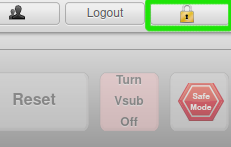
\includegraphics[width=0.46\textwidth]{figs/observing/request.png}
    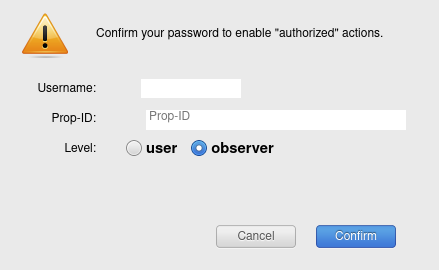
\includegraphics[width=0.49\textwidth]{figs/observing/request_2.png}
    \caption{\textit{Left}: The location to click to begin requesting observer permissions. \textit{Right}: The pop-up window to request observer permissions.}
    \label{fig:request}
\end{figure}

Once you're in, there are a few things you can do. First, update the Observers, Proposal ID, Program, and Investigator information if it hasn't already been updated. You'll find these in the ``System Control'' tab along the top of the screen. Click ``Edit'', edit the text boxes, and then click ``Save''. In the ``Exposure Control'' tab, you upload the actual json scripts. Click ``Load exposure script'', ``Browse...'' and then ``Submit'' (this may appear as ``Sub...''). It'll appear in the exposure queue as a block of yellow, green, or blue exposures. The colors don't mean anything, they're just to differentiate between which exposures belong to which scripts. \\

\begin{figure}
    \centering
    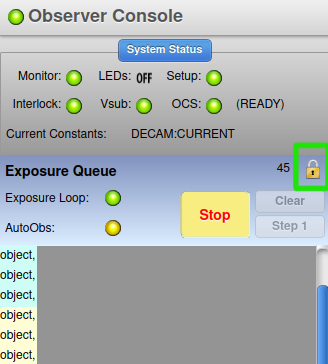
\includegraphics[width=0.5\textwidth]{figs/observing/unlock.png}
    \caption{The exposure queue, with the padlock icon to allow deleting/shuffling of exposures as-needed. Target information from this screenshot is greyed out. To the left of the padlock, ``45'' indicates that there are 45 exposures currently loaded into the queue. Underneath these icons, the ``Stop'' button (which is often red, not yellow, I don't know why it's yellow here) will interrupt the exposure loop. When pressed, it will change to ``Go''. This flip-flops depending on if the exposure loop is running.}
    \label{fig:unlock}
\end{figure}

Once your stuff is in the exposure queue, you can move around or delete the exposures as needed. Click the padlock icon, highlighted in Figure \ref{fig:unlock}, to unfreeze the queue. Now, you can delete things or move them around if you need to. This is uncommon, but it happens. When you're done, \textit{always re-lock it}. To the left of the padlock, there are numbers that switch between integers and a timer. The timer is the amount of exposure time remaining in the queue. The integer is the number of exposures remaining in the queue. \\

In the Telemetry Viewer app, I like to look at the Pointing and Image Health tabs. All plots indicate the values calculated for the \textit{previous} image. They are not updated in real-time. The Pointing tab has pointing and center offsets plots---you'll want to keep an eye on these to make sure these don't drift too far from center. Image Health has a seeing plot, which shows the... seeing. Write this down in your observing log every so often. You don't have to be super precise. This number gets recorded in the FITS header anyway. \\

The Comfort Display SISPI GUI is also important. You should look at all exposures here, in addition to some in the VNC viewer to check for image saturation. If your background counts are $>40,000$, the detector is definitely saturated. \textbf{You must stop saturated observations immediately}. They can damage the instrument. $>20,000$ is maybe not instrument-damaging, but they're a waste of time. Expect the $g-$band to be saturated during bright time, and the $r-$band if you're pointing close to the Moon or have a very long exposure ($>100$s) in bright time. You CAN stop an exposure in the middle and look at counts before continuing if you're concerned it may saturate the detector. \\

You'll want to keep track of the Alarm History GUI as well; if there's a warning, you should figure out what's causing it. Finally, open the Guider app. This will tell you if there are guiding issues, which can arise if you're in a crowded field. \\

% SISPI GUIs that are important: Comfort display (observer should ideally look at ALL exposures that are taken here, plus some on the VNC viewer for e.g. image saturation during bright time), alarm history (you need to know of all warnings and alarms and investigate what's causeing them), guider (so you can see if there are guiding issues e.g. in crowded fields, and keep an eye on ellipticity)

Let's talk about the center offset correction. In the VNC viewer, if a terminal is not already open, open a terminal. Type \texttt{observer}, hit enter, then \texttt{center}, then hit enter. This will print the center offset for the previous image. If it's large, kindly ask your support staff in the Zoom call for a pointing correction. Listen to their instructions about hitting ``Stop'' and ``Go'' in the exposure queue (the correction can't be made in the middle of an exposure---you need to interrupt the exposure loop). I usually ask for a correction around a 10'' offset. If you're near the end of observing an object, don't worry about it, wait until the telescope slews to see if it corrects itself. If not, go ahead and ask.\\

Now that I've said all that, I'll go over using the terminal in the VNC viewer. You'll use a package called Kentools, which you enter in the terminal by typing ``observer''. Exit by typing ``exit''. Like this: 

\begin{minted}[
    bgcolor=lightgray,
    frame=leftline,
    framesep=-3mm]{c}

    # Open Kentools:
    observer2> observer
    # Close Kentools:
    prompt> exit
\end{minted}

That's it! It'll pull up a long list of commands, which I will not copy and paste here. To check centering and seeing, do this: 

\begin{minted}[
    bgcolor=lightgray,
    frame=leftline,
    framesep=-3mm]{c}

    # Open Kentools:
    observer2> observer
    # List commands:
    prompt> commands
    # Check centering for previous image:
    prompt> center
    # Check seeing for the previous image:
    prompt> seeingall
\end{minted}

You can open the images you're taking and look at them in DS9! This is also how you check counts. 

\begin{minted}[
    bgcolor=lightgray,
    frame=leftline,
    framesep=-3mm]{c}

    # From Kentools, check image inventory
    prompt> inv
    # Load the S4 CCD for the previous image (default). 
    prompt> load
\end{minted}

DS9 will pop up with the image. You can check the background counts by hovering your mouse over any location in the image and reading what's in the ``value'' box underneath the ``File'' and ``Object'' information fields.  Here's another example:
\begin{minted}[
    bgcolor=lightgray,
    frame=leftline,
    framesep=-3mm]{c}

    # From Kentools, check image inventory
    prompt> inv
    # I picked exposure number 1156247, and load the N5 CCD. 
    prompt> load 1156247 36
\end{minted}

\begin{figure}[h!]
    \centering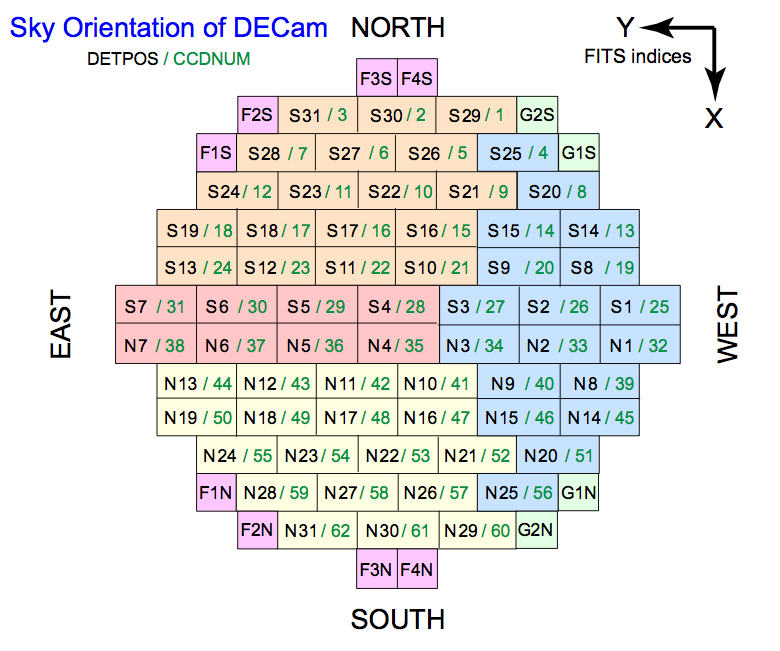
\includegraphics[width=0.8\textwidth]{figs/observing/DECamOrientation.png}
    \caption{Alphanumeric codes for each DECam CCD.}
    \label{fig:decamccds}
\end{figure}

You can get the exposure number from several places. You can type ``inv'' in Kentools to get an inventory of the exposures from that night. The first column is the exposure number. You can also get the most recent exposure number from the dialogue box in the exposure console, or the upper left-hand corner of the comfort display GUI. You can get the CCD code from Figure~\ref{fig:decamccds}. The N5 CCD has a green 36 written next to it, so I type ``36'' to specify that I want to look at that particular CCD. You can also look at the ENTIRE frame with ``bigload''. Same deal as ``load'', but you don't need to specify the CCD because it loads all the CCDs: \texttt{bigload [expnum]}. \\

At the \href{http://www.ctio.noao.edu/noao/content/End-Night-2}{end of the night}, you need to fill out the \href{http://www.ctio.noao.edu/noao/node/add/night-report}{end-of-night report}. If you observed during the first half of the night, you need to create it. If you observed during the second half, you will get the link from the first half observer (unless they didn't start it. Then you need to make it). Get the login credentials from support. It is very important to ask the telescope operator who needs to be reported in the night log! Don't be afraid to ask.\\

% % Antonella comments:
